\section{Results}\label{sec:results}

\subsection{Longer chains change nothing material}
For the 14 models fit both ways, the trial-level elpd changed by at most 1.04 (median 0.37) and the LOSO elpd by at most 0.67 (median 0.30). No pair of models changed order under trial-level LOO, and one pair changed order under LOSO (C+L and C+LMmax, 0.4 apart before and 0.4 after).

The conclusions of the previous report that do not involve the new models therefore stand. All numbers below are from the 5000-draw fits.

\begin{figure}[tbp]
\centering
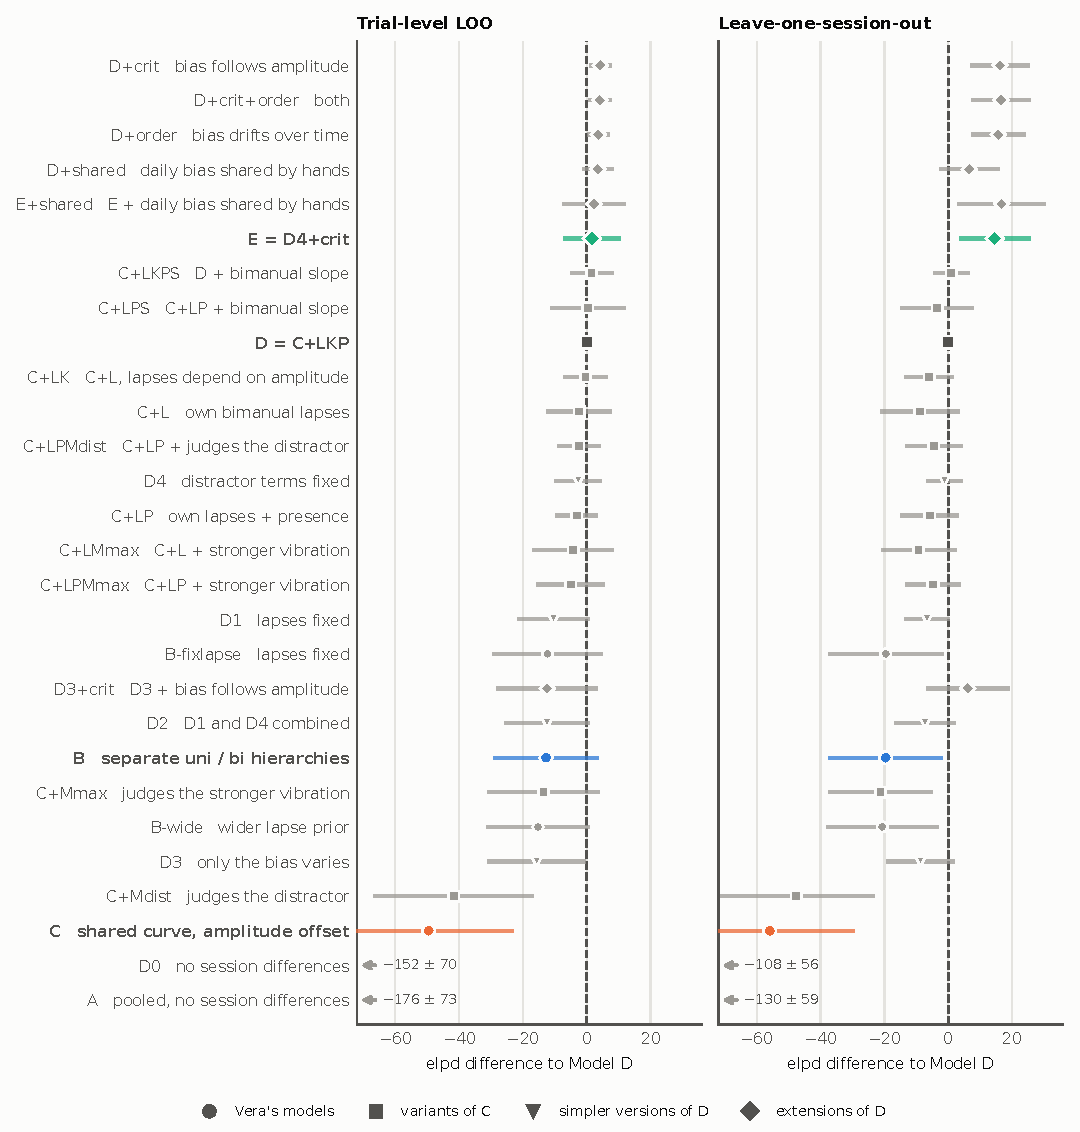
\includegraphics[width=\textwidth]{../results5000/figs/F1_comparison.pdf}
\caption{Predictive performance of every model relative to Model~D (dashed line), with $\pm2$ standard errors; right of the line is better than D.
Left: trial-level LOO, the criterion in Vera's reports, with standard errors from per-session sums.
Right: leave-one-session-out, the accuracy for a session the model has not seen.
Models are sorted by the left panel. B, C and the recommended Model~E are coloured; arrows mark models off the scale.}\label{fig:comparison}
\end{figure}

\begin{table}[p]
\centering\small
\caption{All models, their size and their predictive performance relative to Model~D.
Parameters: hand- or group-level parameters\,/\,parameters per session.
$p_\mathrm{loo}$: effective number of parameters from trial-level LOO.
Differences are in elpd (log-likelihood units summed over all trials); positive means better than D; standard errors in brackets.}\label{tab:comparison}
\setlength{\tabcolsep}{4.5pt}
\begin{tabularx}{\textwidth}{@{}l>{\raggedright\arraybackslash}Xrrr@{\ }lr@{\ }l@{}}
\toprule
Model & What it is & Parameters & $p_\mathrm{loo}$ & \multicolumn{2}{c}{Trial LOO} & \multicolumn{2}{c}{LOSO} \\
 & & pop.\,/\,session & & \multicolumn{2}{c}{vs D (SE)} & \multicolumn{2}{c}{vs D (SE)} \\
\midrule
\multicolumn{8}{@{}l}{\textit{Vera's models}} \\
A & pooled: no session differences & 16\,/\,0 & 13 & \ensuremath{-}176.1 & (36.5) & \ensuremath{-}130.0 & (29.6) \\
B & separate unimanual and bimanual hierarchies & 32\,/\,16 & 179 & \ensuremath{-}12.7 & (8.2) & \ensuremath{-}19.6 & (9.0) \\
B-wide & B with a 3$\times$ wider prior on the lapse sd & 32\,/\,16 & 196 & \ensuremath{-}15.3 & (8.0) & \ensuremath{-}20.7 & (8.8) \\
B-fixlapse & B with lapses fixed per group & 24\,/\,8 & 169 & \ensuremath{-}12.3 & (8.6) & \ensuremath{-}19.6 & (9.0) \\
C & shared curve, bimanual offset $\propto$ amplitude & 20\,/\,10 & 139 & \ensuremath{-}49.5 & (13.3) & \ensuremath{-}55.9 & (13.2) \\
\addlinespace[3pt]
\multicolumn{8}{@{}l}{\textit{Variants of C}} \\
C+L & C + own lapse rates on bimanual trials & 28\,/\,14 & 142 & \ensuremath{-}2.4 & (5.1) & \ensuremath{-}8.9 & (6.2) \\
C+LK & C+L + bimanual lapses depend on amplitude & 32\,/\,14 & 143 & \ensuremath{-}0.4 & (3.5) & \ensuremath{-}6.0 & (3.9) \\
C+LP & C+L + presence offset & 32\,/\,16 & 147 & \ensuremath{-}3.2 & (3.3) & \ensuremath{-}5.8 & (4.5) \\
C+LPS & C+LP + bimanual slope change & 36\,/\,18 & 155 & 0.4 & (5.8) & \ensuremath{-}3.4 & (5.8) \\
C+LKPS & D + bimanual slope change & 40\,/\,18 & 156 & 1.5 & (3.4) & 0.9 & (2.8) \\
C+Mmax & C + judges the stronger vibration & 22\,/\,10 & 134 & \ensuremath{-}13.5 & (8.8) & \ensuremath{-}21.2 & (8.1) \\
C+Mdist & C + judges the distractor & 22\,/\,10 & 135 & \ensuremath{-}41.7 & (12.5) & \ensuremath{-}47.6 & (12.3) \\
C+LMmax & C+L + judges the stronger vibration & 30\,/\,14 & 138 & \ensuremath{-}4.2 & (6.3) & \ensuremath{-}9.3 & (5.9) \\
C+LPMmax & C+LP + judges the stronger vibration & 34\,/\,16 & 141 & \ensuremath{-}5.0 & (5.3) & \ensuremath{-}4.8 & (4.2) \\
C+LPMdist & C+LP + judges the distractor & 34\,/\,16 & 141 & \ensuremath{-}2.4 & (3.4) & \ensuremath{-}4.5 & (4.4) \\
\addlinespace[3pt]
\multicolumn{8}{@{}l}{\textit{Model D, recommended in the previous report}} \\
\textbf{D (= C+LKP)} & C+LK + presence offset & 36\,/\,16 & 145 & 0 &  & 0 &  \\
\addlinespace[3pt]
\multicolumn{8}{@{}l}{\textit{Simpler versions of D}} \\
D4 & D, distractor terms fixed per hand & 32\,/\,12 & 125 & \ensuremath{-}2.7 & (3.7) & \ensuremath{-}1.2 & (2.8) \\
D1 & D, lapses fixed per hand and condition & 28\,/\,8 & 130 & \ensuremath{-}10.4 & (5.7) & \ensuremath{-}6.7 & (3.6) \\
D2 & D1 and D4 combined & 24\,/\,4 & 109 & \ensuremath{-}12.4 & (6.7) & \ensuremath{-}7.2 & (4.8) \\
D3 & D2 + slope fixed: only the bias varies & 22\,/\,2 & 88 & \ensuremath{-}15.7 & (7.6) & \ensuremath{-}8.7 & (5.3) \\
D0 & D with no session differences & 20\,/\,0 & 18 & \ensuremath{-}152.0 & (35.2) & \ensuremath{-}108.2 & (28.2) \\
\addlinespace[3pt]
\multicolumn{8}{@{}l}{\textit{Extensions of D}} \\
D+shared & D + daily bias shared by the two hands & 37\,/\,17 & 141 & 3.5 & (2.4) & 6.6 & (4.7) \\
D+crit & D + bias follows the distractor amplitude & 38\,/\,16 & 144 & 4.2 & (1.8) & 16.2 & (4.6) \\
D+order & D + bias drifts over the study & 38\,/\,16 & 144 & 3.7 & (1.8) & 15.7 & (4.3) \\
D+crit+order & D + both & 40\,/\,16 & 144 & 4.1 & (1.8) & 16.6 & (4.7) \\
\addlinespace[3pt]
\multicolumn{8}{@{}l}{\textit{Simpler versions with the trend}} \\
\textbf{E (= D4+crit)} & D4 + bias follows the distractor amplitude & 34\,/\,12 & 123 & 1.6 & (4.5) & 14.6 & (5.6) \\
D3+crit & D3 + bias follows the distractor amplitude & 24\,/\,2 & 84 & \ensuremath{-}12.4 & (7.9) & 6.1 & (6.5) \\
E+shared & E + daily bias shared by the two hands & 35\,/\,13 & 121 & 2.3 & (4.9) & 16.7 & (6.9) \\
\bottomrule
\end{tabularx}

\end{table}

\subsection{Model D beats Vera's models, and why}
Model~D predicts better than Model~B by both scores (Fig.~\ref{fig:comparison}, Table~\ref{tab:comparison}):
by \DvsBTrial\ (SE \DvsBTrialSE) at the trial level and by \DvsBLoso\ (SE \DvsBLosoSE) for new sessions, where it predicts \DvsBLosoNbetter\ of the 42 held-out sessions better.
It does this with fewer effective parameters ($p_\mathrm{loo}$ \plooD\ against \plooB), because it ties the unimanual and bimanual trials of a hand to one curve instead of fitting them separately.
Model~C is far behind both (D minus C: \DvsCTrial\ $\pm$ \DvsCTrialSE\ at the trial level, \DvsCLoso\ $\pm$ \DvsCLosoSE\ for new sessions).

The variants of C show which parts of D matter.
\begin{itemize}
\item Giving bimanual trials their own lapse rates (C+L) is the largest single step: \LvsCTrial\ over C at the trial level. C+L alone already beats B (\LvsBTrial\ $\pm$ \LvsBTrialSE; new sessions \LvsBLoso\ $\pm$ \LvsBLosoSE).
\item Letting those lapse rates change with the distractor amplitude and adding the presence offset helps most for new sessions: D minus C+L is \DvsLTrial\ $\pm$ \DvsLTrialSE\ at the trial level and \DvsLLoso\ $\pm$ \DvsLLosoSE\ for new sessions.
\item A change of slope on bimanual trials adds nothing (D with a bimanual slope, minus D: \SvsDTrial\ at the trial level, \SvsDLoso\ for new sessions).
\item Capture by the stronger vibration explains much of C's deficit with one parameter per hand (\MmaxvsCTrial\ over C), but adds nothing once the lapses are per condition (\LMmaxvsLTrial\ $\pm$ \LMmaxvsLTrialSE\ over C+L at the trial level). Replacing D's amplitude-dependent lapses by capture of the distractor (C+LPMdist: on a fraction $\pi$ of bimanual trials Sirius judges the distractor) does slightly worse than D (\CapturevsDTrial\ $\pm$ \CapturevsDTrialSE\ at the trial level, \CapturevsDLoso\ $\pm$ \CapturevsDLosoSE\ for new sessions), and puts capture on only \piCapturePctLeft\% (left) and \piCapturePctRight\% (right) of bimanual trials.
\item Widening the prior on B's lapse variation does not help B (\BwidevsBTrial\ at the trial level, \BwidevsBLoso\ for new sessions), and fixing B's lapses across sessions makes no difference (\BfixvsBTrial\ at the trial level, \BfixvsBLoso\ for new sessions).
\end{itemize}

The raw counts show what B and C miss (Fig.~\ref{fig:ppc}).
For weak targets (6--12\um) Sirius answered ``high'' on 81 of 1,606 bimanual trials (5.0\%) but on only 4 of 1,627 unimanual trials (0.25\%).
Strong targets (44--50\um) drew ``low'' on 2.0\% of trials in both conditions.
The bimanual excess differs between the hands.
For the left hand it appears only with strong distractors: none in 262 trials of the 6 and 12\um\ sessions, 36 of 447 (8.1\%) in the 24--32\um\ sessions.
For the right hand it is about 5\% at every distractor amplitude.
Model~C has one pair of lapse rates for both conditions, so it cannot produce twenty times more weak-target errors on bimanual trials.
Model~B gives bimanual trials their own lapse rates but cannot tie them to the distractor: it pulls every session toward a common rate, so for the left hand it predicts \ppcLowAmpPredB\% ``high'' answers in the 6--12\um\ sessions, where there were none.
In D the bimanual lapse rate changes with the session's distractor amplitude.
For the left hand the ``high'' lapse rises steeply with amplitude ($\kappa_h=\kappaHDLeft$, 95\% interval \kappaHDLeftLo\ to \kappaHDLeftHi, on the logit scale per 14.6\um); for the right hand it barely changes ($\kappa_h=\kappaHDRight$, \kappaHDRightLo\ to \kappaHDRightHi).
In posterior predictive checks of these error rates by hand and amplitude the observed rate falls inside the 95\% predictive interval in \ppcInD\ of \ppcN\ cells for D, \ppcInE\ for E, \ppcInB\ for B and \ppcInC\ for C.
Figure~\ref{fig:byamp} shows where the gains over B come from: the sessions with the weakest distractors and the 24--30\um\ sessions. In the 32\um\ sessions B still fits slightly better at the trial level, but not for new sessions.

\begin{figure}[tbp]
\centering
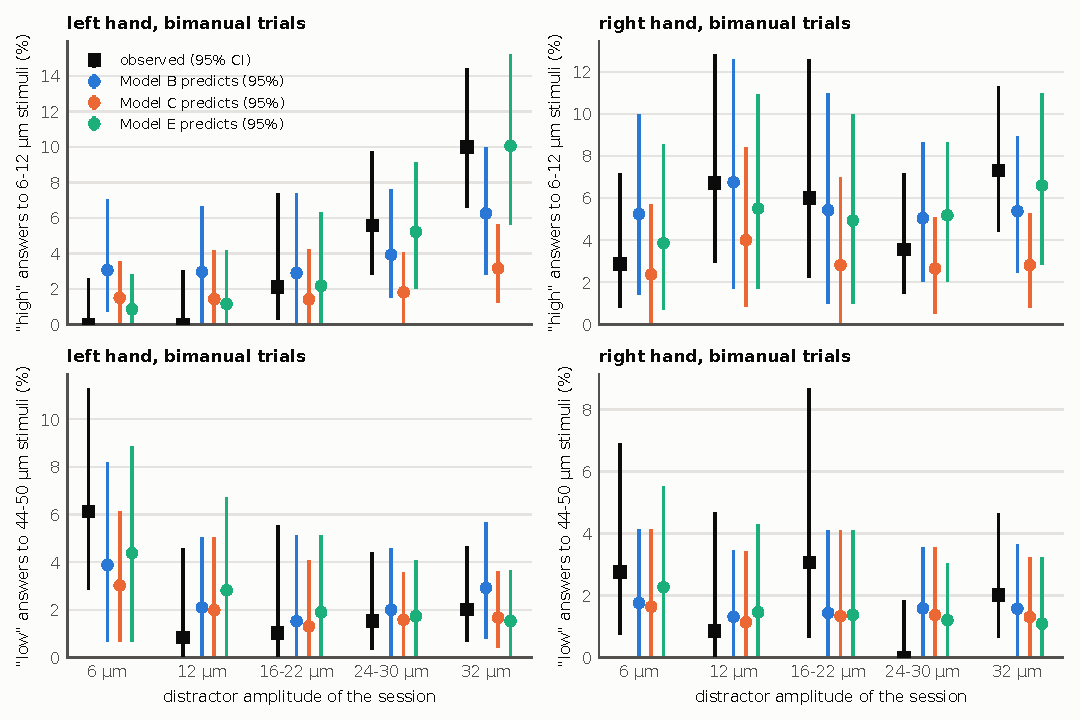
\includegraphics[width=\textwidth]{../results5000/figs/F3_lapse_ppc.pdf}
\caption{Lapse-like answers on bimanual trials, by hand and by the session's distractor amplitude: ``high'' answers to the two weakest targets (top) and ``low'' answers to the two strongest (bottom).
Black: observed rate with a 95\% binomial interval. Coloured: each model's posterior predictive mean and 95\% interval.}\label{fig:ppc}
\end{figure}

\begin{figure}[tbp]
\centering
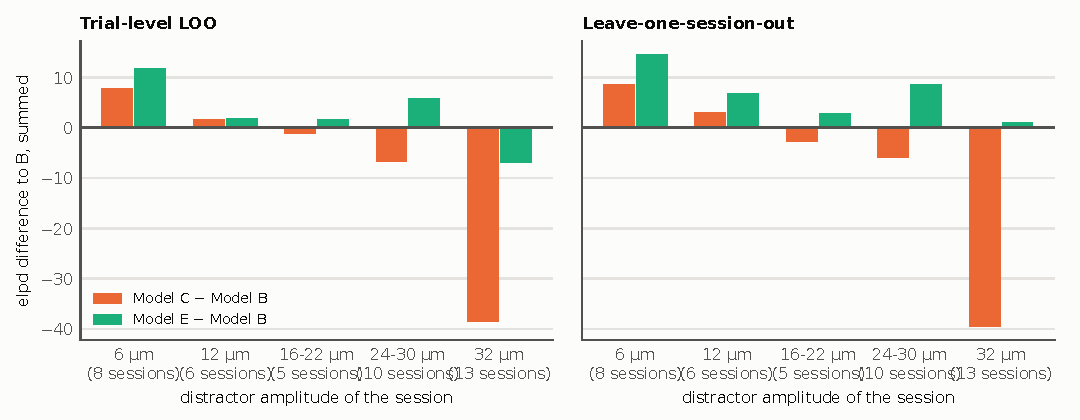
\includegraphics[width=\textwidth]{../results5000/figs/F5_vs_B_by_amplitude.pdf}
\caption{Where Models C and E gain or lose against Model~B, summed over the sessions with each distractor amplitude. Positive: better than B.}\label{fig:byamp}
\end{figure}

\subsection{Extensions: Sirius's criterion moved over the study}\label{sec:ext}
Model~D gives every session its own bias, but it treats the sessions as interchangeable: it expects no order in them.
There is order (Fig.~\ref{fig:time}).
Sirius's unimanual PSE rose over the study, most clearly for the right hand: it called fewer unimanual targets ``high'' in the later sessions, which were also the sessions with the strongest distractors.

Two extensions describe this with one extra parameter per hand.
In \textbf{D+crit} the session bias follows the session's distractor amplitude; in \textbf{D+order} it drifts linearly with the session's place in the study.
\begin{itemize}
\item Both predict clearly better than D, above all for new sessions: D+crit by \CritvsDTrial\ $\pm$ \CritvsDTrialSE\ at the trial level and \CritvsDLoso\ $\pm$ \CritvsDLosoSE\ for new sessions (better on \CritvsDLosoNbetter\ of 42), D+order by \OrdervsDTrial\ $\pm$ \OrdervsDTrialSE\ and \OrdervsDLoso\ $\pm$ \OrdervsDLosoSE.
No other single addition to D comes close; the next best, a shared daily bias, gains \SharedvsDLoso\ for new sessions.
\item The two cannot be told apart. D+crit minus D+order is \CritvsOrderTrial\ $\pm$ \CritvsOrderTrialSE\ at the trial level and \CritvsOrderLoso\ $\pm$ \CritvsOrderLosoSE\ for new sessions. A model with both terms is no better than either (\CritOrdervsCritLoso\ $\pm$ \CritOrdervsCritLosoSE\ over D+crit), and in it neither coefficient is clearly different from zero.
The design does not allow the distinction: the distractor amplitude was raised steadily, so it is correlated 0.91 with the session order. Only the four 24\um\ sessions run late in the study break the pattern, and they do not settle it: three lean slightly towards drift and one towards adaptation (together $-1.5$ elpd for D+crit against D+order).
\item The size of the change: in a typical session the unimanual PSE is \critPseLeft\um\ higher in the 32\um\ sessions than in the 6\um\ sessions for the left hand (95\% interval \critPseLeftLo\ to \critPseLeftHi) and \critPseRight\um\ higher for the right (\critPseRightLo\ to \critPseRightHi), comparable to the bimanual shift itself.
For the left hand the rise roughly offsets the distractor's push: the overall proportion of ``high'' answers to left-hand targets stays between 0.44 and 0.49 in every amplitude group, while unimanual ``high'' answers fall from 0.44 to 0.39 and bimanual ones rise from 0.45 to 0.54. For the right hand the criterion rose further than that.
\end{itemize}

Modelling the trend changes one conclusion of the previous report.
When every session's bias is pulled toward a single value (Model~D), part of the trend is absorbed by the bimanual terms, because the bias is shared by a session's unimanual and bimanual trials.
With the trend modelled, the bimanual shift grows more steeply with amplitude ($b_2=\muBtwoCritLeft$ left and \muBtwoCritRight\ right, against \muBtwoDLeft\ and \muBtwoDRight\ in D) and the presence offset shrinks.
For the right hand it remains clear ($b_3=\muBthreeCritRight$, \muBthreeCritRightLo\ to \muBthreeCritRightHi); for the left hand it is no longer distinguishable from zero (\muBthreeCritLeft, \muBthreeCritLeftLo\ to \muBthreeCritLeftHi).
The shift averaged over sessions, the JND result and the lapse pattern do not change (Table~\ref{tab:effects}).

\paragraph{A shared daily bias}
The two hands' session biases are correlated (0.50 between their unimanual PSEs in Model~D, 0.36 to 0.41 after a linear trend in amplitude or time is removed). A daily offset shared by the hands (D+shared) improves on D (\SharedvsDTrial\ $\pm$ \SharedvsDTrialSE\ at the trial level, \SharedvsDLoso\ $\pm$ \SharedvsDLosoSE\ for new sessions), but much less than the trend does for new sessions (D+shared minus D+crit: \SharedvsCritLoso\ $\pm$ \SharedvsCritLosoSE): much of what the hands share from day to day is the trend. Added to E, the shared offset is small ($\sigma_v=\sigSharedEshared$ on the logit scale) and gains little (\EsharedvsETrial\ $\pm$ \EsharedvsETrialSE\ at the trial level, \EsharedvsELoso\ $\pm$ \EsharedvsELosoSE\ for new sessions).

\begin{figure}[tbp]
\centering
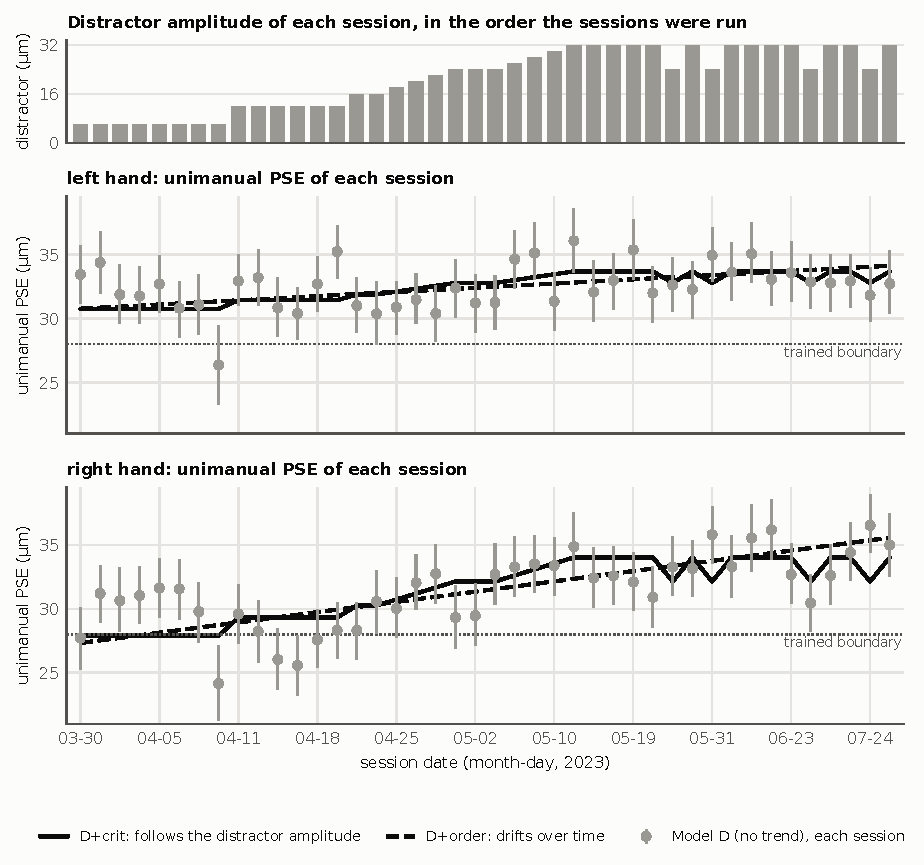
\includegraphics[width=\textwidth]{../results5000/figs/F6_bias_time_amplitude.pdf}
\caption{Top: the distractor amplitude of each session, in the order the sessions were run.
Middle and bottom: each session's unimanual PSE in Model~D, which assumes no trend (grey, 95\% intervals), with the typical-session PSE of the two extensions:
the bias follows the distractor amplitude (D+crit, solid) or drifts linearly over time (D+order, dashed).
Both lines track the rise; only the four late 24\um\ sessions could separate them.}\label{fig:time}
\end{figure}


\subsection{Simpler models: only the bias and the lapses need to vary between sessions}\label{sec:simpler}
Model~D lets eight parameters per hand vary from session to session. The simpler versions hold some of them fixed (Fig.~\ref{fig:complexity}, Table~\ref{tab:comparison}).
\begin{itemize}
\item \textbf{The bias must vary.} With no session differences at all, D0 minus D is \DzerovsDTrial\ at the trial level.
\item \textbf{The distractor terms need not vary.} Holding $b_2$ and $b_3$ fixed for each hand (D4 minus D: \DfourvsDTrial\ $\pm$ \DfourvsDTrialSE\ at the trial level, \DfourvsDLoso\ $\pm$ \DfourvsDLosoSE\ for new sessions) saves 4 parameters per session and 20 effective parameters (\plooD\ $\to$ \plooDfour). Once its amplitude is taken into account, the distractor has the same effect in every session.
\item \textbf{Neither, largely, does the slope.} Holding it fixed as well changes little (D3 minus D2: \DthreevsDtwoTrial\ $\pm$ \DthreevsDtwoTrialSE\ at the trial level, \DthreevsDtwoLoso\ $\pm$ \DthreevsDtwoLosoSE\ for new sessions).
\item \textbf{The lapse rates do vary.} Holding them fixed loses ground (D1 minus D: \DonevsDTrial\ $\pm$ \DonevsDTrialSE\ at the trial level, \DonevsDLoso\ $\pm$ \DonevsDLosoSE\ for new sessions), and this step accounts for most of what the simpler models D2 and D3 lose.
\end{itemize}

The same simplifications hold with the criterion trend.
\textbf{Model~E} (D4+crit: bias, slope and lapses vary between sessions, the distractor terms are fixed per hand, and the bias follows the distractor amplitude) is as good as D+crit (E minus D+crit: \DfourCritvsCritTrial\ $\pm$ \DfourCritvsCritTrialSE\ at the trial level, \DfourCritvsCritLoso\ $\pm$ \DfourCritvsCritLosoSE\ for new sessions) with 20 fewer effective parameters (\plooDfourCrit\ against \plooCrit).
It beats D by \DfourCritvsDLoso\ $\pm$ \DfourCritvsDLosoSE\ and B by \DfourCritvsBLoso\ $\pm$ \DfourCritvsBLosoSE\ for new sessions.
Even D3+crit, with a single bias per hand and session (2 parameters per session against 16 in B and D), predicts new sessions as well as D (\DthreeCritvsDLoso\ $\pm$ \DthreeCritvsDLosoSE) and better than B (\DthreeCritvsBLoso\ $\pm$ \DthreeCritvsBLosoSE), with fewer than half of B's effective parameters (\plooDthreeCrit\ against \plooB).

\begin{figure}[tbp]
\centering
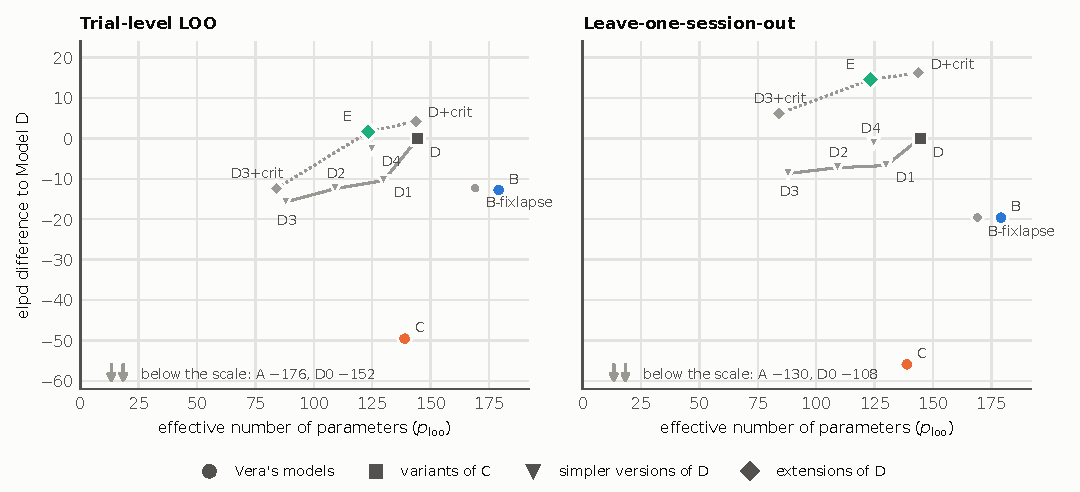
\includegraphics[width=\textwidth]{../results5000/figs/F2_complexity.pdf}
\caption{Predictive performance against model complexity (effective number of parameters, $p_\mathrm{loo}$), relative to Model~D (dashed line).
Solid grey line: the simpler versions of D, from D3 (only the bias varies between sessions) through D2 and D1 to D.
Dotted grey line: the same with the criterion trend, from D3+crit through E to D+crit.}\label{fig:complexity}
\end{figure}


\subsection{The distractor effects in the recommended model}
Every model that predicts well gives the same picture of the distractor's effect on the point of subjective equality (PSE, the target amplitude judged ``high'' half the time; Table~\ref{tab:effects}, Fig.~\ref{fig:shift}).
\begin{itemize}
\item On bimanual trials the PSE moves down. Averaged over sessions, the shift in Model~E is \ShiftDfourCritLeft\um\ for the left hand (95\% interval \ShiftDfourCritLeftLo\ to \ShiftDfourCritLeftHi) and \ShiftDfourCritRight\um\ for the right (\ShiftDfourCritRightLo\ to \ShiftDfourCritRightHi). A distractor makes the target feel stronger.
\item The shift grows with distractor amplitude, from \ShiftSixDfourCritLeft\um\ in the 6\um\ sessions to \ShiftThirtytwoDfourCritLeft\um\ in the 32\um\ sessions for the left hand, and from \ShiftSixDfourCritRight\ to \ShiftThirtytwoDfourCritRight\um\ for the right.
\item The right hand is shifted even by a weak distractor: its presence offset is $b_3=\muBthreeDfourCritRight$ (\muBthreeDfourCritRightLo\ to \muBthreeDfourCritRightHi), against \muBthreeDfourCritLeft\ (\muBthreeDfourCritLeftLo\ to \muBthreeDfourCritLeftHi) for the left.
\item There is no reliable change in sensitivity. Model~B's increase of the left hand's JND, \JndBLeft\um\ (\JndBLeftLo\ to \JndBLeftHi), shrinks to \JndDfourCritLeft\um\ in E, and that remainder comes from the bimanual lapses, which flatten the curve's ends, not from a change of slope. With a free bimanual slope the increase is \JndSLeft\um, but the slope change itself is uncertain ($\mu_\delta=\muDboneSLeft$, \muDboneSLeftLo\ to \muDboneSLeftHi) and does not improve prediction.
\end{itemize}

\begin{table}[tbp]
\centering\small
\caption{Distractor effects in \textmu m (posterior mean and 95\% interval): the mean over all sessions, or over the sessions with a 6 or a 32\um\ distractor. PSE shift: bimanual minus unimanual PSE; JND change: bimanual minus unimanual JND. In C the two curves differ only by a shift, so its JND change is zero by construction.}\label{tab:effects}
\setlength{\tabcolsep}{4pt}
\begin{tabular}{@{}llcccc@{}}
\toprule
Quantity (\textmu m) & Hand & B & C & D & E \\
\midrule
PSE shift, mean & left & \ensuremath{-}4.3 [\ensuremath{-}5.1, \ensuremath{-}3.5] & \ensuremath{-}4.5 [\ensuremath{-}5.1, \ensuremath{-}3.8] & \ensuremath{-}4.0 [\ensuremath{-}4.8, \ensuremath{-}3.3] & \ensuremath{-}4.0 [\ensuremath{-}4.7, \ensuremath{-}3.3] \\
 & right & \ensuremath{-}6.1 [\ensuremath{-}6.8, \ensuremath{-}5.3] & \ensuremath{-}5.7 [\ensuremath{-}6.4, \ensuremath{-}5.1] & \ensuremath{-}6.0 [\ensuremath{-}6.7, \ensuremath{-}5.2] & \ensuremath{-}5.9 [\ensuremath{-}6.7, \ensuremath{-}5.3] \\
\addlinespace[2pt]
PSE shift, 6\,\textmu m & left & \ensuremath{-}1.1 [\ensuremath{-}2.7, 0.5] & \ensuremath{-}1.3 [\ensuremath{-}1.8, \ensuremath{-}0.9] & \ensuremath{-}1.8 [\ensuremath{-}3.3, \ensuremath{-}0.5] & \ensuremath{-}1.4 [\ensuremath{-}2.7, \ensuremath{-}0.1] \\
 & right & \ensuremath{-}3.9 [\ensuremath{-}5.3, \ensuremath{-}2.1] & \ensuremath{-}1.8 [\ensuremath{-}2.2, \ensuremath{-}1.4] & \ensuremath{-}4.2 [\ensuremath{-}5.6, \ensuremath{-}2.9] & \ensuremath{-}3.6 [\ensuremath{-}5.0, \ensuremath{-}2.3] \\
\addlinespace[2pt]
PSE shift, 32\,\textmu m & left & \ensuremath{-}6.6 [\ensuremath{-}8.0, \ensuremath{-}5.4] & \ensuremath{-}7.4 [\ensuremath{-}8.5, \ensuremath{-}6.3] & \ensuremath{-}5.7 [\ensuremath{-}6.8, \ensuremath{-}4.5] & \ensuremath{-}6.1 [\ensuremath{-}7.2, \ensuremath{-}5.0] \\
 & right & \ensuremath{-}7.9 [\ensuremath{-}9.0, \ensuremath{-}6.7] & \ensuremath{-}8.6 [\ensuremath{-}9.7, \ensuremath{-}7.5] & \ensuremath{-}7.4 [\ensuremath{-}8.5, \ensuremath{-}6.3] & \ensuremath{-}7.7 [\ensuremath{-}8.7, \ensuremath{-}6.6] \\
\addlinespace[2pt]
JND change, mean & left & 1.0 [0.5, 1.6] & 0 (by design) & 0.3 [0.2, 0.5] & 0.4 [0.2, 0.5] \\
 & right & 0.5 [0.0, 1.1] & 0 (by design) & 0.2 [0.1, 0.3] & 0.2 [0.1, 0.4] \\
\bottomrule
\end{tabular}

\end{table}

\begin{figure}[tbp]
\centering
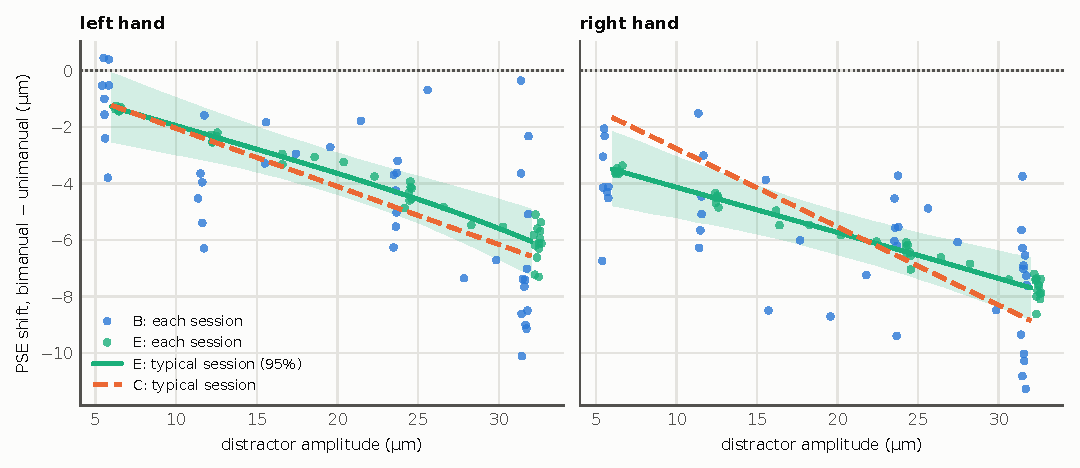
\includegraphics[width=\textwidth]{../results5000/figs/F4_shift_vs_amplitude.pdf}
\caption{PSE shift (bimanual minus unimanual) against the session's distractor amplitude. Dots: each session's estimate in Models B and E. Lines: a typical session in E (with 95\% interval) and in C.
C forces the shift to be proportional to amplitude; E allows a presence offset, which the right hand needs.}\label{fig:shift}
\end{figure}
